V práci \cite{A_scoping_review_of_gaze_and_eye_tracking-based_control_methods_for_assistive_robotic_arms} autori identifikovali tri hlavné kategórie prístupov k ovládaniu asistívnych robotických ramien pomocou pohľadu, a to systémy založené na telemanipulácii, metódy využívajúce smerový pohľad na riadenie pohybu robota a objektovo orientované stratégie, pri ktorých používateľ výberom objektu pohľadom iniciuje autonómne alebo poloautonómne akcie robota.

Táto práca zároveň zistila, že medzi jednotlivými technikami ovládania sa najčastejšie využíva fixácia pohľadu, keďže predstavuje najstabilnejší a najľahšie detekovateľný signál zámeru používateľa. Autori však upozorňujú aj na tzv. „Midas touch“ problém, pri ktorom môže neúmyselná fixácia vyvolať neželanú akciu robota, čo predstavuje významnú prekážku pre spoľahlivé a bezpečné ovládanie. V rámci analýzy existujúcich riešení zároveň autori identifikovali viaceré kľúčové výzvy, medzi ktoré patrí potreba zlepšenia presnosti sledovania očí v rôznych svetelných podmienkach, minimalizácia chýb spôsobených pohybom hlavy či posunom zariadenia, zabezpečenie prirodzenej a intuitívnej interakcie bez preťaženia používateľa a taktiež nedostatok štandardizovaných metód hodnotenia výkonu týchto systémov, ktoré by umožnili spoľahlivo porovnávať výsledky naprieč štúdiami.

\subsubsection{Telemanipulácia}
Telemanipulácia podľa článku \cite{A_scoping_review_of_gaze_and_eye_tracking-based_control_methods_for_assistive_robotic_arms} predstavuje spôsob ovládania asistívneho robotického ramena, pri ktorom používateľ pomocou pohľadu interaguje s grafickým rozhraním a prostredníctvom výberu ikon, tlačidiel či smerových príkazov manuálne riadi jednotlivé pohyby robota. Ide o plne používateľom kontrolovaný proces, bez autonómnych zásahov systému, kde každý krok manipulácie musí byť explicitne iniciovaný fixáciou pohľadu.

Tento princíp sa objavuje vo viacerých analyzovaných štúdiách, hoci každá z nich realizuje telemanipuláciu trochu odlišne. V článku \cite{Eye-tracking-based_robotic_arm_control_system} bol systém navrhnutý okolo jednoduchého panelu s ôsmimi príkazovými políčkami určujúcimi pohyb ramena v šiestich smeroch a ovládanie koncového chápadla. Používateľ vždy fixoval jeden z ponúkaných príkazov, ktorý bol následne okamžite vykonaný robotickým ramenom. Súčasťou rozhrania bol aj živý obraz z kamery umiestnenej na robotickom ramene (vid. Obrázok~\ref{fig:gui-control-system}), čo uľahčovalo priestorovú orientáciu a presnejšie vykonávanie úloh.

\begin{figure}[H]
    \centering
    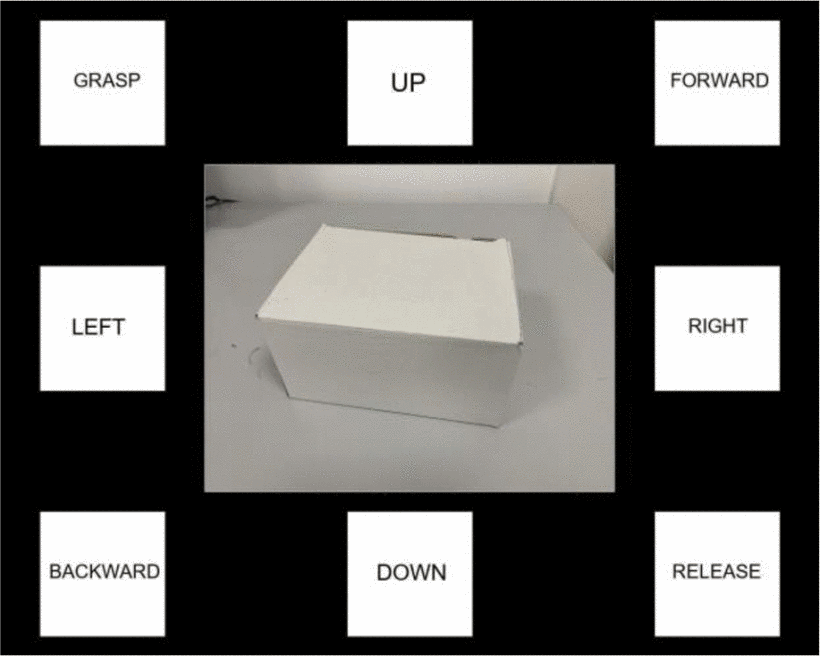
\includegraphics[width=0.75\textwidth]{images/control-system.png}
    \caption{Grafické používateľské rozhranie s ôsmimi príkazovými políčkami a živým obrazom z kamery umiestnenej na robotickom ramene, prevzaté z \cite{Eye-tracking-based_robotic_arm_control_system}.}
    \label{fig:gui-control-system}
\end{figure}

V štúdii \cite{Eye-gaze_control_of_a_wheelchair_mounted_6DOF_assistive_robot_for_activities_of_daily_living} autori rozšírili koncept telemanipulácie o komplexnejšie používateľské rozhranie, keďže robotické rameno bolo integrované priamo na invalidnom vozíku a bolo potrebné zabezpečiť ovládanie viacerých funkcií súčasne. Grafické používateľské rozhranie bolo rozdelené do viacerých funkčných sekcií, pričom každá z nich umožňovala odlišný typ manipulácie (vid. Obrázok~\ref{fig:gui-withwheelchair}). Horná časť rozhrania obsahovala prepínanie medzi operačnými režimami, napríklad medzi kartézskym ovládaním v rovine X–Y alebo režimom určeným pre robot umiestnený na vozíku. V centrálnej časti sa nachádzal hlavný panel so smerovými tlačidlami, ktorý umožňoval pohyb ramena vpred, vzad, doľava, doprava, nahor a nadol. Pri týchto prvkoch boli zároveň umiestnené príkazy na ovládanie koncového chápadla (z ang. gripper), teda príkazy na uchopenie a uvoľnenie objektu. Spodná časť rozhrania bola venovaná práci s preddefinovanými úlohami ADL, kde bolo možné načítať uložené sekvencie, spustiť ich alebo sa vrátiť do predchádzajúcej ponuky. Pravá časť rozhrania slúžila na detailné ovládanie jednotlivých stupňov voľnosti robotického ramena, pričom používateľ výberom pohľadu určoval orientáciu a nastavenia šiestich kĺbov.

\begin{figure}[H]
    \centering
    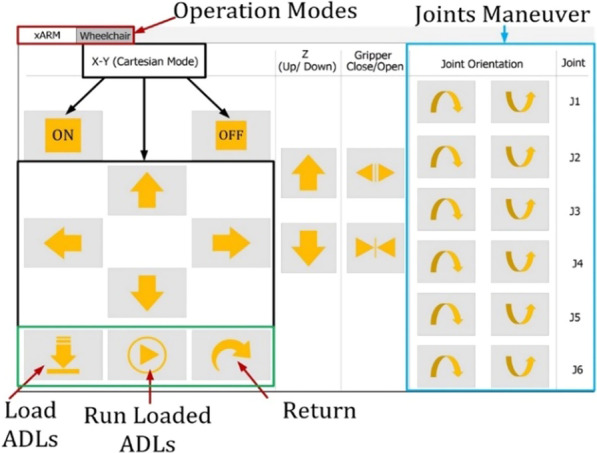
\includegraphics[width=0.9\textwidth]{images/with-wheelchair.jpg}
    \caption{Grafické používateľské rozhranie systému pre ovládanie robotického ramena pomocou sledovania pohľadu, prevzaté z \cite{Eye-gaze_control_of_a_wheelchair_mounted_6DOF_assistive_robot_for_activities_of_daily_living}.}
    \label{fig:gui-withwheelchair}
\end{figure}

Podobný princíp bol použitý aj v práci \cite{Implementation_and_performance_comparison_for_two_versions_of_eye_tracking_based_robotic_arm_movement}, kde bol systém navrhnutý tak, aby používateľ ovládal všetkých šesť stupňov voľnosti robotického ramena prostredníctvom rozhrania so zreteľne označenými tlačidlami (vid. Obrázok~\ref{fig:gui-comparison}). Softvér sledovania očí mapoval pohyb očí na pohyb kurzora a fixácia pohľadu na konkrétnom tlačidle generovala signál odoslaný do Raspberry Pi, ktoré následne riadilo servomotory ramena. Tak ako v predchádzajúcich prácach, aj tu nebol prítomný žiadny autonómny prvok, teda robot reagoval výhradne na sériu postupných očných príkazov.

\begin{figure}[H]
    \centering
    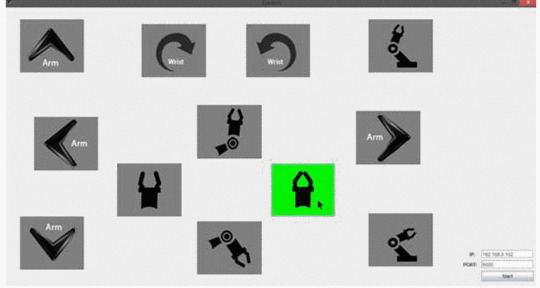
\includegraphics[width=0.9\textwidth]{images/comparison.jpg}
    \caption{Grafické používateľské rozhranie systému pre ovládanie robotického ramena pomocou sledovania pohľadu, prevzaté z \cite{Implementation_and_performance_comparison_for_two_versions_of_eye_tracking_based_robotic_arm_movement}.}
    \label{fig:gui-comparison}
\end{figure}

Telemanipulačný princíp bol prítomný aj v systéme EMOHEX \cite{EMOHEX:_An_eye_tracker_based_mobility_and_hand_exoskeleton_device_for_assisting_disabled_people}, kde sa pomocou sledovania pohľadu ovládala kombinácia elektrického vozíka a ručného exoskeletonu. Na rozdiel od predchádzajúcich štúdií však exoskeleton nemal priestorový pohyb, vykonával iba úchopové akcie (uchop, drž, pusť), zatiaľ čo pohyb k objektu zabezpečoval samotný vozík. Používateľ ovládal dve prepínateľné ovládacie panely, jeden určený na navigáciu vozíka a druhý na ovládanie prstového exoskeletonu (vid. Obrázok~\ref{fig:gui-emohex}).

\begin{figure}[H]
    \centering
    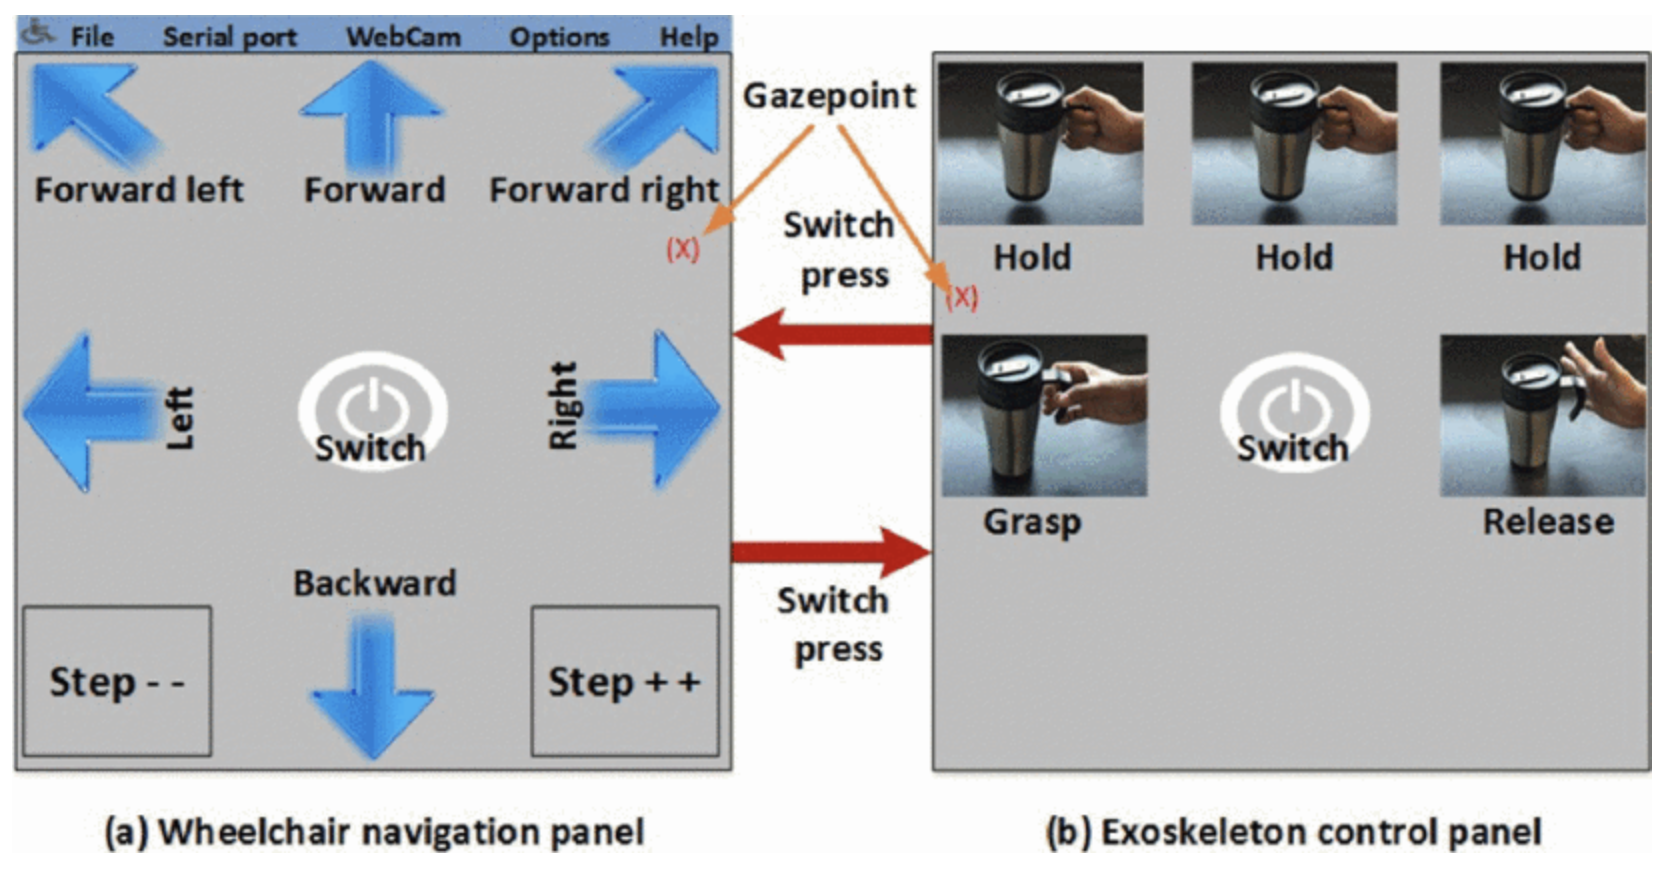
\includegraphics[width=0.9\textwidth]{images/emohex.png}
    \caption{Grafické používateľské rozhranie systému pre ovládanie robotického ramena a invalidného vozíka pomocou sledovania pohľadu, prevzaté z \cite{EMOHEX:_An_eye_tracker_based_mobility_and_hand_exoskeleton_device_for_assisting_disabled_people}.}
    \label{fig:gui-emohex}
\end{figure}

Telemanipulačný prístup bol použitý aj v práci \cite{Eye_Gaze_Controlled_Robotic_Arm_for_Persons_with_Severe_Speech_and_Motor_Impairment}, kde autori navrhli priehľadné rozhranie umožňujúce ovládanie robotického ramena výhradne pomocou fixácie pohľadu. Systém pozostával zo snímača očí, tabletu zobrazujúceho živý obraz z kamery a robotického ramena ovládaného servomotormi. Na obrazovke boli v reálnom čase prekryté transparentné ovládacie oblasti, na ktoré používateľ fixoval pohľad a tým vydával príkazy. Pri úlohe zdvihni a polož boli okolo objektu a cieľovej polohy vykreslené zelené rámčeky, fixácia pohľadu na rámček dlhšia než 500 ms automaticky spustila uchopenie objektu, pričom ďalšia fixácia vykonala jeho položenie.

\begin{figure}[H]
    \centering
    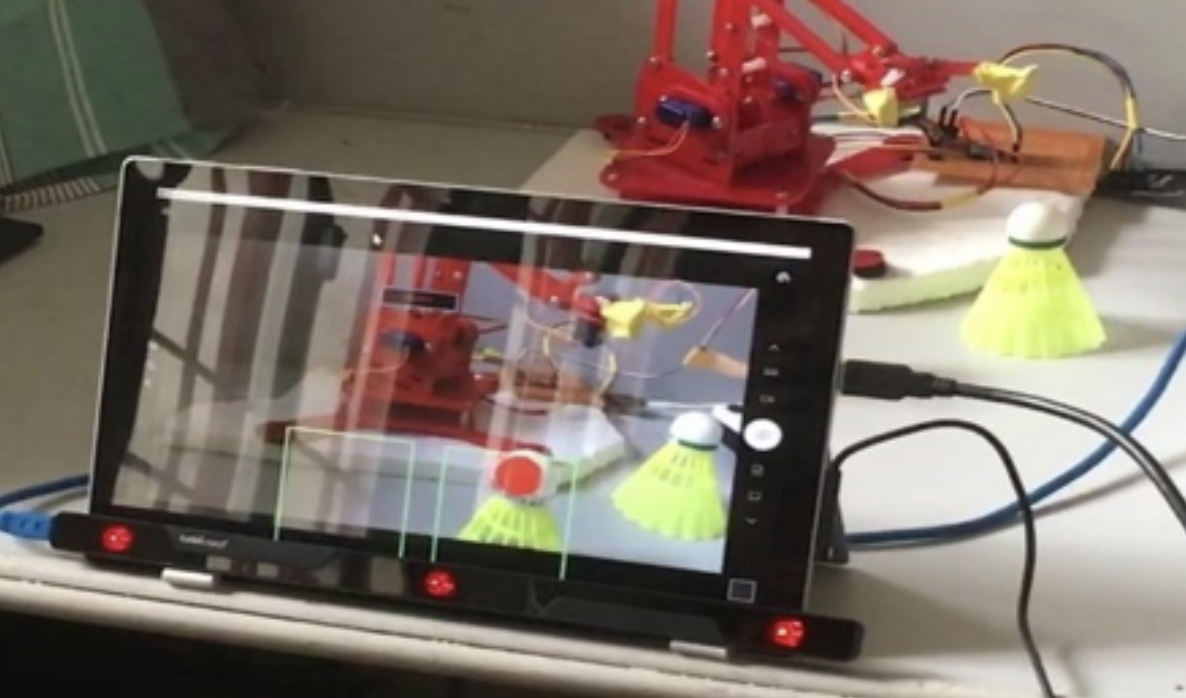
\includegraphics[width=0.9\textwidth]{images/see-through.png}
    \caption{Transparetné rozhranie z \cite{Eye_Gaze_Controlled_Robotic_Arm_for_Persons_with_Severe_Speech_and_Motor_Impairment}.}
    \label{fig:see-through}
\end{figure}

\subsubsection{Smerový pohľad}
Podľa článku \cite{A_scoping_review_of_gaze_and_eye_tracking-based_control_methods_for_assistive_robotic_arms} predstavuje ovládanie asistívneho robotického ramena smerovým pohľadom prístup, pri ktorom používateľ nevyberá objekt, ale iba udáva smer pohybu robota tým, kam sa pozerá. Softvér teda nespracúva výber cieľového predmetu, či fixáciu na ikonách, ale interpretuje orientáciu očí ako priamy príkaz na vykonanie konkrétnej akcie.

Príklad takéhoto prístupu ponúka práca \cite{Persistent_Human–Machine_Interfaces_for_Robotic_Arm_Control_Via_Gaze_and_Eye_Direction_Tracking}, ktorá predstavila ľudské-strojové rozhranie umožňujúce ovládanie robotického ramena výhradne na základe smeru pohľadu. Systém využíva dvojkamerové sledovanie očí (webkamera a komerčný snímač očí) a hlbokú konvolučnú neurónovú sieť (CNN), ktorá klasifikuje štyri základné pohyby očí: pohľad hore, pohľad vľavo, pohľad vpravo a žmurknutie. Tieto akcie sú potom namapované na príkazy robota, napríklad pohľad hore spúšťa pohyb ramena vpred, pohľad vľavo aktivuje režim uchopenia, vpravo režim uvoľnenia a žmurknutie slúži ako stop alebo potvrdenie príkazu. CNN bola trénovaná na stovkách obrazov očí a dosiahla extrémne vysokú presnosť 99,99 percent v reálnom čase, čo umožnilo spoľahlivé ovládanie robotického ramena aj pri veľmi jemných pohyboch očí. Ovládanie robota prebieha tak, že CNN klasifikuje pohyb oka ako priamy príkaz, zatiaľ čo samotný bod pohľadu slúži na výber regiónu či pracovnej oblasti, do ktorej má robot ruku nasmerovať. Výsledkom je hybridný systém schopný vykonať až 64 rôznych príkazov bez potreby grafického rozhrania alebo výberu objektov.

\subsubsection{Objektovo orientovaný pohľad}
V článku \cite{A_scoping_review_of_gaze_and_eye_tracking-based_control_methods_for_assistive_robotic_arms} bol objektovo orientovaný pohľad (z ang. object-oriented gaze) opísaný tak, že používateľ fixuje pohľad priamo na objekt, s ktorým chce interagovať a systém potom rozpozná tento objekt, vypočíta v 3D priestore jeho pozíciu a automaticky (alebo poloautomaticky) vykoná manipulačnú akciu robota bez toho, aby používateľ musel explicitne zadávať smer alebo príkaz.

V štúdii \cite{Proof_of_Concept_of_an_Assistive_Robotic_Arm_Control_Using_Artificial_Stereovision_and_Eye-Tracking} autori predstavili systém PoGARA, ktorý umožňuje ovládanie asistívneho robotického ramena výhradne pomocou pohľadu používateľa v reálnom 3D prostredí. Na rozdiel od telemanipulačných systémov, ktoré vyžadujú manuálne zadávanie jednotlivých smerových príkazov prostredníctvom grafického rozhrania, tu používateľ vykonáva iba jediný krok, pozrie sa na objekt, ktorý chce uchopiť. Softvér sledovania očí sníma smer pohľadu a stereovízna kamera vytvára 3D model scény ako voxelovú mapu (z ang. Voxel grid). Voxelová mapa je 3D digitálna mapa prostredia, ktorá prostredie rozdeľuje na malé voxely. Voxel predstavuje malý objemový prvok v trojrozmernom priestore a môže mať jeden zo stavov: obsadený, voľný alebo neznámy. Kombináciou týchto dvoch vstupov systém vypočíta presnú priestorovú súradnicu, kam používateľ sa pozerá.

Po identifikovaní cieľového objektu systém automaticky vykoná celý proces manipulácie. Najprv pomocou algoritmu A* vypočíta kolízne bezpečnú trajektóriu pre robotické rameno, pričom využíva voxelovú mapu prostredia. Následne pomocou reverzných a priamych kinematík zabezpečí, aby sa robotické rameno vyhlo všetkým objektom v scéne vrátane prekážok. Kinematika robotického ramena popisuje vzťah medzi polohou kĺbov a polohou koncového chápadla. Priama kinematika vypočíta polohu a orientáciu koncového chápadla na základe toho, v akých uhloch sú jednotlivé kĺby. Reverzná kinematika rieši opačný problém, vypočíta, aké uhly kĺbov musí robotické rameno nastaviť, aby sa koncové chápadlo dostalo na požadované miesto.

V článku \cite{GazeGrasp:_DNN-Driven_Robotic_Grasping_with_Wearable_Eye-Gaze_Interface} autori predstavili systém GazeGrasp, ktorý taktiež využíva objektovo orientovaný prístup k ovládaniu robotického ramena, avšak v kombinácii s pokročilými metódami počítačového videnia. Používateľ ovláda robotické rameno prostredníctvom nositeľného snímača očí zabudovaného do okuliarov, ktoré snímajú pohyb očí pomocou kamery (Obrázok ~\ref{fig:gazegrasp}a). Pred samotným používaním systém vyžaduje kalibráciu, počas ktorej sa používateľ pozerá na 35 preddefinovaných bodov na obrazovke. Zo zaznamenaných súradníc dúhovky sa pomocou polynomiálnej regresie vytvorí model, ktorý následne presne mapuje smer pohľadu na súradnice obrazovky a umožňuje spoľahlivú interpretáciu vizuálnych príkazov. Na obrazovke počítača sa zároveň zobrazuje živý obraz z kamery umiestnenej na koncovom chápadle robota (Obrázok ~\ref{fig:gazegrasp}c). V tomto obraze sú objekty v pracovnom priestore automaticky detegované pomocou hlbokej neurónovej siete YOLOv8, ktorá ich identifikuje a zvýrazní ohraničujúcimi rámčekmi (Obrázok ~\ref{fig:gazegrasp}b),. YOLOv8 je moderná konvolučná neurónová sieť trénovaná na rozsiahlych datasetoch s miliónmi anotovaných obrázkov, čo jej umožňuje spoľahlivo rozpoznávať širokú škálu objektov aj v dynamických alebo neideálnych svetelných podmienkach. Model vytvára ohraničujúce rámčeky okolo detegovaných objektov, odhaduje ich pozíciu v obraze a poskytuje aj skóre istoty detekcie. Vďaka tomu systém dokáže stabilne identifikovať predmety, s ktorými má robot manipulovať, a zároveň minimalizovať falošné detekcie. Používateľ si objekt volí jednoducho tým, že sa naň pozrie, pričom fixácia pohľadu na jeden z detegovaných objektov po dobu troch sekúnd spustí proces uchopenia.

Systém navyše využíva takzaný efekt magnetického zameriavania (z ang. magnetic snapping), pri ktorom sa kurzor riadený pohľadom automaticky presunie do stredu ohraničovacieho rámčeka objektu, ak sa pohľad používateľa dostane do jeho vnútra. Tento mechanizmus výrazne znižuje náročnosť presného zamierenia pohľadu na malé objekty a podľa výsledkov experimentu skracuje čas potrebný na zarovnanie pohľadu o viac než 30 percent. Po voľbe objektu systém automaticky prepočíta súradnice objektu z obrazového priestoru do súradnicového priestoru robota pomocou transformačných matíc medzi kamerou a robotickou základňou. Robotické rameno potom autonómne pristúpi k objektu a uchopí ho pomocou koncového chápadla. Rovnakým spôsobom používateľ vyberá aj cieľové miesto, kam má robot objekt umiestniť, stačí, aby sa pozrel na prázdnu oblasť pracovného priestoru a pohľad na ňu podržal.

\begin{figure}[H]
    \centering
    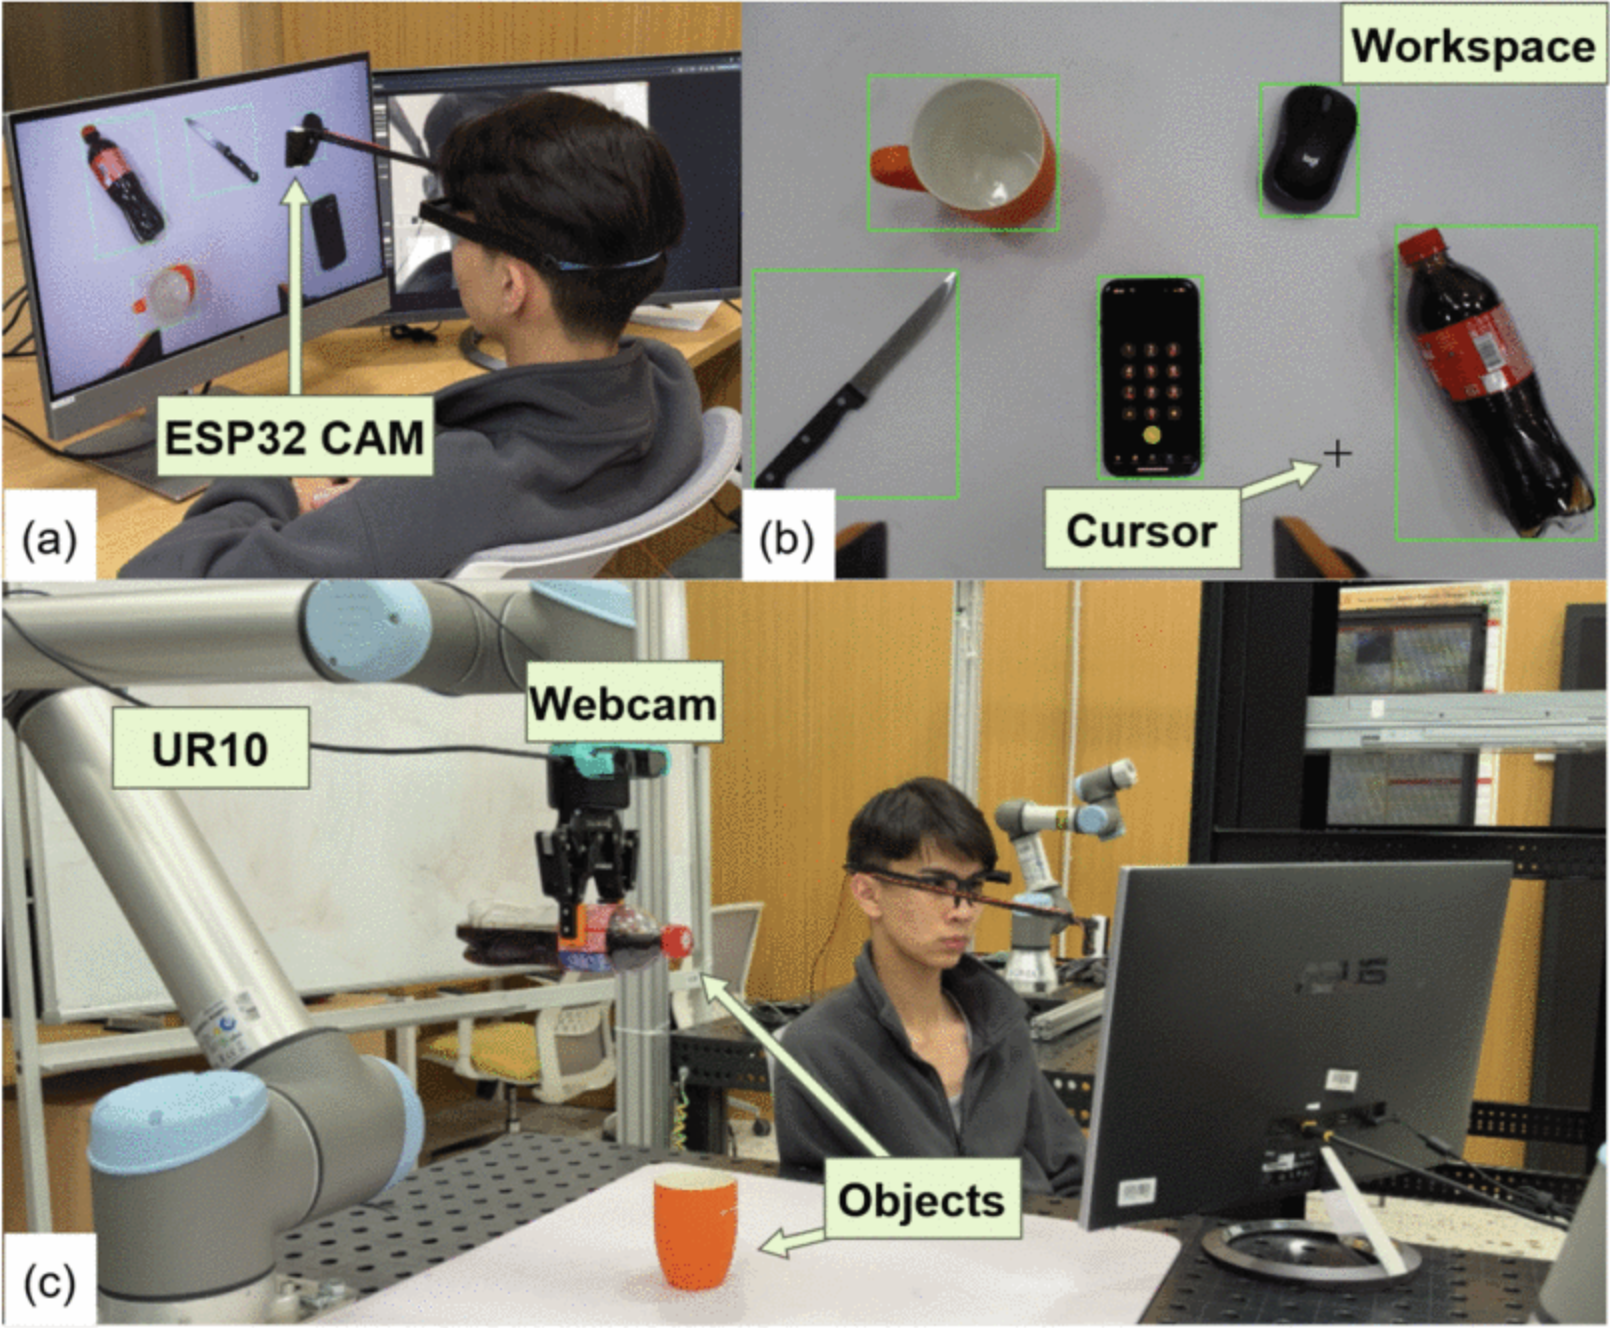
\includegraphics[width=0.9\textwidth]{images/gazegrasp.png}
    \caption{Ukážka systému GazeGrasp z \cite{GazeGrasp:_DNN-Driven_Robotic_Grasping_with_Wearable_Eye-Gaze_Interface}.}
    \label{fig:gazegrasp}
\end{figure}

V článku \cite{Robotic_arm_control_by_augmented_reality-assisted_object_detection} autori predstavili pokročilý systém ovládania asistívneho robotického ramena, ktorý kombinuje sledovanie pohľadu, rozšírenú realitu (AR) a objektovú detekciu v reálnom čase. HoloLens2 so vstavaným snímaním očí zaznamenáva pohľad používateľa a zároveň pomocou svojich RGB kamier a priestorového mapovania vytvára 3D reprezentáciu okolia. Objekty v pracovnom priestore sú automaticky detegované pomocou ľahkej verzie hlbokej siete YOLOv8n, pričom ich polohy sú vizualizované v AR prostredí formou 3D ohraničujúcich rámčekov.

Používateľ vyberá objekt výhradne pohľadom, ak sa na príslušný rámček pozerá súvisle počas piatich sekúnd, systém ho považuje za cieľ a následne spustí autonómny proces manipulácie. Na rozdiel od telemanipulačných systémov tak používateľ nemusí zadávať žiadne smerové ani krokové príkazy. Po potvrdení výberu systém vykoná tzv. ray-casting z HoloLens2 smerom k stredu vybraného rámčeka, čím presne určí 3D súradnice objektu v priestore. Poloha robotického ramena je získaná pomocou jednorazového skenovania QR kódu, ktorý definuje jeho referenčný rámec v prostredí. Na základe relatívnej pozície robot následne autonómne naplánuje pohyb, zarovná koncový efektor a objekt uchopí.

Po uchopení objektu sa v AR zobrazí interaktívne rozhranie s tromi voľbami. Prvá funkcia privedie uchopený predmet k ústam používateľa, pričom ich poloha je dynamicky odhadovaná pomocou priestorového sledovania HoloLens2. Druhá funkcia umožňuje sekundárnu manipuláciu objektu v piatich smeroch, čo je užitočné napríklad na odsunutie prekážok v scéne. Tretia funkcia ukončí úlohu a robot vráti objekt do pôvodnej polohy.